\section{VeriFast}

Im Rahmen dieser Seminararbeit werden wir uns hauptsächlich mit dem Verifikationswerkzeug \emph{VeriFast} auseinandersetzen, dass in Form eines Prototypen an der KU Leuven ins Leben gerufen wurde und bis heute, Stand 2018, aktiv weiterentwickelt wird. VeriFast erlaubt die Verifikation von \emph{single-} und \emph{multithreaded} C und Java Programmen, welche mit zusätzlichen Annotationen, für die Verifikation bestimmter Korrektheitseigenschaften, ausgestattet sind. Die Annotationen stehen dabei innerhalb von Kommentaren, wodurch der verifizierte C Code ohne zusätzliche Änderungen kompiliert werden kann. Während der Ausführung von VeriFast wird das Programm auf illegale Speicherzugriffe, beispielsweise durch Dereferenzierung von Null-Pointern oder durch Zugriff auf Speicherzellen außer der Grenzen eines Arrays, sowie Fehler aufgrund nebenläufiger Ausführung geprüft. Darüber hinaus untersucht VeriFast die annotierten Methoden-Kontrakte - d.h. es wird versucht zu zeigen, dass sich die spezifizierte Nachbedingung aus der Vorbedingung und der symbolischen Ausführung des Methodenrumpfs ableiten lässt. \cite{Jacobs2010}

\begin{figure}[!hbt]
	\centering
	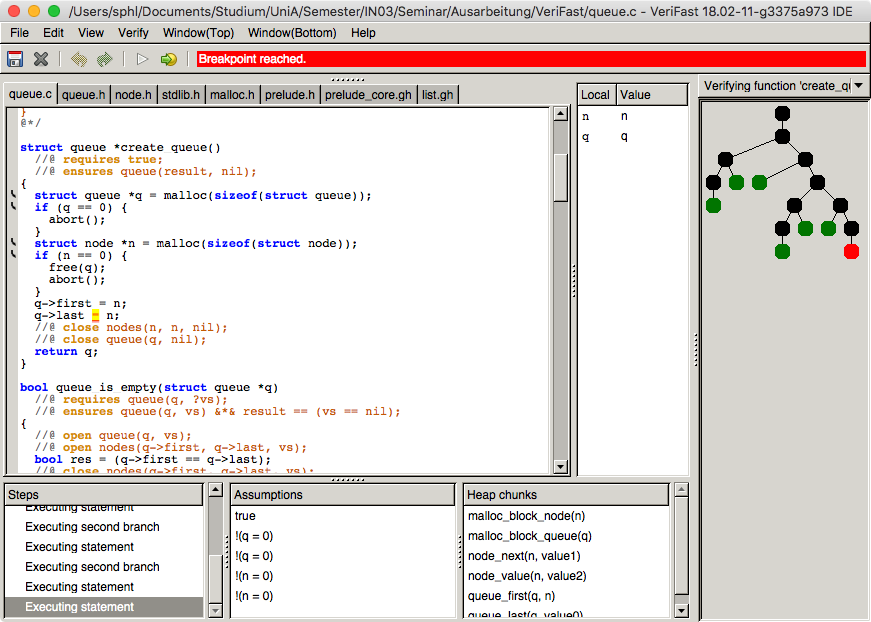
\includegraphics[width=0.8\linewidth]{verifast}
	\caption{VeriFast IDE}
	\label{fig:vfide}
\end{figure}

\noindent
Über die VeriFast IDE (siehe \vref{fig:vfide}) können Quellcodedateien modifiziert und Programme schrittweise oder in einem Durchlauf verifiziert werden. Im Falle eines Fehlers werden diese innerhalb des Editors lokalisiert und anhand einer Statusmeldung dem Benutzer mitgeteilt. Wurde die Verifikation erfolgreich durchlaufen, so können abhängig von der ausgewählten Funktion die getesteten Pfade in Form eines Ausführungsbaums am rechten Fensterrand angezeigt werden. Dieser erlaubt es, durch anklicken eines Blattknotens, einzelne Pfad genauer zu untersuchen. Die \emph{Steps}-Auswahl (unten links) listet dabei die ausgeführten Schritte eines Pfades auf und erlaubt Sprünge zu vorherigen bzw. nachfolgenden Zuständen. In dem Auswahlfenster nebenan befinden sich die logischen Annahmen, die sich dynamisch zur Ausführung aus den Annotationen und dem C Code ergeben. Eine weitere Besonderheit der IDE sind die \emph{heap chunks} (unten rechts), welche den symbolischen Zustand des Heap-Speichers abhängig von den Ausführungsschritt anzeigt. Direkt neben dem Editor befindet sich eine weitere Auswahl, welche einen Überblick über die Zuordnung der lokalen Variablen auf deren symbolischen Werte gibt. \cite{Jacobs2017}

\subsection{Sprachkonstrukte}

\subsubsection{Induktive Datentypen}

\subsubsection{malloc\_block Einheiten}

\subsubsection{Prädikate}

\subsubsection{Fixpunkt Funktionen}

\subsubsection{Lemma Funktionen}

\subsubsection{Kontrakte}

\subsubsection{Schleifeninvarianten}

\subsection{Verifikation -- Binärsuche}

\subsection{Praxis Fallstudien}

\subsubsection{Embedded Linux Network Management Software}

\subsubsection{Linux USB BP Keyboard Driver}

\subsection{Fazit}